\documentclass[tikz]{standalone}

\usepackage{circuitikz}

\begin{document}
	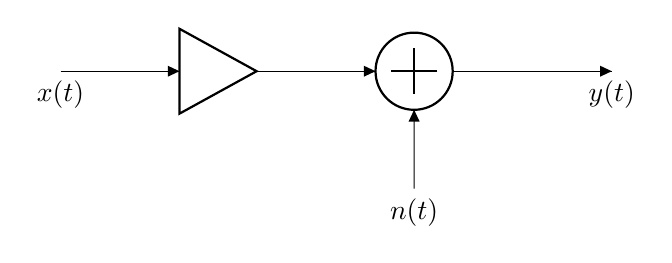
\begin{tikzpicture}
		\draw (0,0) node[below]{$x(t)$} to[amp, >] (4,0)
            node[adder, anchor=west](adder){};
        \node [inputarrow, anchor=tip] at (adder.west) {};
        \draw (adder.east) to[short] (7,0) node[inputarrow]{} node[below]{$y(t)$};
        \draw (adder.south) to[short] ++(0,-1) node[below]{$n(t)$};
        \node [inputarrow, anchor=tip, rotate=90] at (adder.south) {};
	\end{tikzpicture}
\end{document}